\chapter{Stage 01: study design and the five data sources}
\label{ch:stage01}

Stage~01 of your workflow answers three questions: \emph{where} (Kanha), \emph{when} (two matched dry seasons) and \emph{with what} (five data sources). This chapter explains each, together with the remote-sensing ideas you need to describe them correctly.

\section{Where: Kanha Tiger Reserve and the study rectangle}
\label{sec:studyarea}

\subsection{The reserve}

Kanha Tiger Reserve lies in the Maikal hills of central India, in the Mandla and Balaghat districts of Madhya Pradesh. Its core zone covers 917.44\,km$^2$ and its buffer zone 1,134.36\,km$^2$, 2,051.79\,km$^2$ in total \citep{kanha2026}. The forests are dominated by sal (\emph{Shorea robusta}), with moist peninsular sal forest, southern tropical moist mixed deciduous forest and dry deciduous mixed forest, interspersed with grassland meadows \citep{kanha2026}. Most rain falls in the June--September monsoon; January and February are cool and dry.

\begin{whybox}
The dataset handbook (\file{EcoExplain-VLM_Dataset_Creation_Handbook.docx}, Chapter~3) compared Kanha with Pench and Achanakmar and chose Kanha because it is large enough for 300--500 non-overlapping patches, has varied forest types and a documented disturbance history (fire, encroachment, management), has little cloud in the dry season, and has been studied a lot. The roadmap asked for ``one geographically compact forest area'' so that ecological variation stays limited; one reserve satisfies that.
\end{whybox}

\subsection{The study rectangle}

The code does not use the official reserve boundary. It uses a rectangle (\file{configs/pilot_kanha.yaml}, \file{data/raw_metadata/roi.geojson}):
\[
80.433^\circ\text{E} \le \text{longitude} \le 81.050^\circ\text{E}, \qquad 22.117^\circ\text{N} \le \text{latitude} \le 22.450^\circ\text{N}.
\]
Earth Engine reports its area as 2,350.7\,km$^2$ (notebook 01, cell 4). That is larger than the reserve (2,051.8\,km$^2$), so some patches may lie in the buffer zone or just outside the official boundary.

\begin{watchout}
The config file calls the rectangle ``Kanha official boundary''. It is not the official boundary; it is a box around the reserve. In the report, say ``a rectangle enclosing Kanha Tiger Reserve'' and give its corners.
\end{watchout}

\section{When: matched dry-season windows}

\begin{table}[H]
\centering
\begin{tabular}{lll}
\toprule
Window & Dates & Role \\
\midrule
T0 (before) & 1 January--28 February 2022 & first observation \\
T1 (after) & 1 January--28 February 2023 & second observation, same months \\
Climatology & 2015--2021 & baseline for the ERA5-Land anomalies \\
\bottomrule
\end{tabular}
\end{table}

\emph{Phenology} is the yearly cycle of plant life: leaf flush, full canopy, leaf fall. Kanha's deciduous forests are greenest after the monsoon and lose leaves through the dry season. If the two windows came from different seasons, every patch would show a large NDVI change caused by the season alone. Taking the \emph{same two months} in both years removes most of that effect; the roadmap calls this ``matched seasonal windows''.

\begin{whybox}
January--February is dry and mostly cloud-free in central India and comes before the main leaf fall. The handbook first proposed November--February; the narrower window mixes fewer stages of leaf fall into each composite. One year apart is long enough for clearing or fire to show.
\end{whybox}

\begin{watchout}
Matching the months does not remove differences between years. January--February 2023 was much drier and warmer than 2022 across the whole region (rain fell from about 69 to 25\,mm; Section~\ref{sec:climate}). Leaves dry and fall earlier in such a year, so part of the region-wide NDVI drop may be early seasonal drying, not forest loss. Write ``vegetation decline signal'', not ``degradation'' or ``deforestation''.
\end{watchout}

\section{Remote sensing in five ideas}

You need these five ideas to describe the data sources correctly. Keep them short in the report (one or two sentences with a citation); this section is for your understanding.

\subsection{Passive and active sensors}

Remote sensing means measuring something without touching it; here, satellites record energy coming from the ground. \textbf{Passive} sensors record reflected sunlight: Sentinel-2 is passive, so it sees nothing at night or through cloud. \textbf{Active} sensors send their own signal and record the echo: Sentinel-1 is a radar, so it works at night and through cloud. The project uses both on purpose: optical data say most about leaves and greenness; radar adds structure and moisture \citep{lillesand2015}.

\subsection{Rasters, pixels and bands}

A \textbf{raster} is a grid of numbers laid over the ground. Each cell is a \textbf{pixel} covering a fixed square of land (10\,m\,$\times$\,10\,m for Sentinel-2's sharpest bands). A satellite image is a stack of such grids, one per wavelength range; each grid is a \textbf{band}. A \textbf{GeoTIFF} is an image file that also records where on Earth the grid lies. The position system is the \textbf{coordinate reference system} (CRS); this project's files use EPSG:4326, latitude and longitude in degrees (Chapter~\ref{ch:stage02} explains why that matters).

\subsection{Four kinds of resolution}

\begin{description}
  \item[Spatial] Ground size of a pixel: Sentinel-2 10--20\,m, Sentinel-1 10\,m, NASADEM 30\,m, CHIRPS about 5.5\,km, ERA5-Land about 9--11\,km.
  \item[Spectral] Which wavelengths, and how many bands. Sentinel-2 has 13 bands; the project exports 10.
  \item[Temporal] How often the same place is seen: Sentinel-2 every 5 days with two satellites; Sentinel-1 every 12 days per satellite.
  \item[Radiometric] How finely brightness is recorded: Sentinel-2 uses 12 bits (4,096 levels).
\end{description}

\begin{plainwords}
A 640\,m patch holds about 4,500 Sentinel-2 pixels but sits inside a \emph{single} CHIRPS or ERA5-Land pixel. So rainfall and temperature describe the surrounding region, not the patch itself. This one fact explains several results later on.
\end{plainwords}

\subsection{From digital numbers to surface reflectance}

The satellite records \emph{digital numbers}. Processing turns them into \emph{reflectance}: the fraction of incoming sunlight that is reflected, from 0 to 1. Level-1C products give top-of-atmosphere reflectance, which still includes haze and aerosols. Level-2A products give \textbf{surface reflectance}, with the atmosphere removed by ESA's Sen2Cor processor; the project uses these (\texttt{COPERNICUS/S2\_SR\_HARMONIZED}). Earth Engine stores reflectance multiplied by 10,000:
\begin{equation}
\rho = \frac{\mathrm{DN}}{10\,000}.
\end{equation}

\begin{whybox}
Surface reflectance is the right input for comparing two years, because the atmosphere is different on every date. On 25 January 2022 ESA changed the Sentinel-2 processing baseline and added an offset of 1,000 to the stored values; the T0 window straddles that date. Earth Engine's \texttt{\_HARMONIZED} collection removes the offset so that scenes before and after the change are comparable. One sentence about this in your Methods shows care.
\end{whybox}

\subsection{Composites}

Each window contains many scenes. A \textbf{composite} combines them into one image per window. The project takes the per-pixel \textbf{median}: for every pixel, the middle value over all clear observations. A missed cloud (too bright) or shadow (too dark) on one date is then ignored. The cost is that a composite is not a single moment; it represents typical conditions in January--February.

\section{Source 1: Sentinel-2 optical imagery}

Sentinel-2 is part of the European Copernicus programme \citep{drusch2012}. Two satellites (2A from 2015, 2B from 2017) carry the MultiSpectral Instrument with a 290\,km swath.

\begin{table}[H]
\centering
\caption{The ten Sentinel-2 bands exported for every patch (\texttt{S2\_OPTICAL\_BANDS} in \file{src/gee_utils.py}). Centre wavelengths are approximate.}
\label{tab:s2bands}
\small
\begin{tabular}{llrrl}
\toprule
Band & Name & Centre (nm) & Pixel (m) & Used for \\
\midrule
B2 & Blue & 490 & 10 & colour image, EVI \\
B3 & Green & 560 & 10 & colour image \\
B4 & Red & 665 & 10 & colour image, NDVI, EVI \\
B5, B6, B7 & Red edge 1--3 & 705--783 & 20 & stored only \\
B8 & Near infrared (NIR) & 842 & 10 & NDVI, EVI, NDMI, NBR \\
B8A & Narrow NIR & 865 & 20 & stored only \\
B11 & Short-wave infrared 1 & 1610 & 20 & NDMI \\
B12 & Short-wave infrared 2 & 2190 & 20 & NBR \\
\bottomrule
\end{tabular}
\end{table}

\subsection{Why leaves look the way they do to a satellite}

Chlorophyll absorbs blue and red light for photosynthesis, so healthy leaves reflect little red. The cell structure inside leaves scatters near-infrared strongly, so healthy canopies reflect 30--50\,\% of NIR. Water in leaves absorbs short-wave infrared, so SWIR reflectance rises when leaves dry out or burn. Every vegetation index below uses these contrasts \citep{tucker1979}.

\subsection{Cloud masking}

Two steps remove cloud (\texttt{mask\_s2\_clouds} in \file{src/gee_utils.py}): a scene filter keeps scenes whose \texttt{CLOUDY\_PIXEL\_PERCENTAGE} is below 20\,\%; then a pixel mask removes cloud shadow, medium- and high-probability cloud, thin cirrus and snow using the Scene Classification Layer (SCL) that comes with every Level-2A scene. After masking, the medians use 20 scenes for T0 and 23 for T1 (notebook 01, cell 6).

\subsection{The four vegetation indices}

All four indices are \emph{normalised differences}: a difference divided by a sum, which keeps values between $-1$ and $+1$ and cancels much of the effect of overall brightness.

\begin{align}
\mathrm{NDVI} &= \frac{\rho_{\mathrm{NIR}} - \rho_{\mathrm{Red}}}{\rho_{\mathrm{NIR}} + \rho_{\mathrm{Red}}} = \frac{B8 - B4}{B8 + B4} \label{eq:ndvi}\\[3pt]
\mathrm{EVI} &= 2.5\,\frac{\rho_{\mathrm{NIR}} - \rho_{\mathrm{Red}}}{\rho_{\mathrm{NIR}} + 6\rho_{\mathrm{Red}} - 7.5\rho_{\mathrm{Blue}} + 1} \label{eq:evi}\\[3pt]
\mathrm{NDMI} &= \frac{\rho_{\mathrm{NIR}} - \rho_{\mathrm{SWIR1}}}{\rho_{\mathrm{NIR}} + \rho_{\mathrm{SWIR1}}} = \frac{B8 - B11}{B8 + B11} \label{eq:ndmi}\\[3pt]
\mathrm{NBR} &= \frac{\rho_{\mathrm{NIR}} - \rho_{\mathrm{SWIR2}}}{\rho_{\mathrm{NIR}} + \rho_{\mathrm{SWIR2}}} = \frac{B8 - B12}{B8 + B12} \label{eq:nbr}
\end{align}

\begin{description}
  \item[NDVI] Proposed by \citet{rouse1974} and popularised by \citet{tucker1979}. Dense healthy vegetation gives about 0.6--0.9, bare soil about 0.1, water below 0; in this dataset the 2022 patch means range from 0.44 to 0.80. NDVI \emph{saturates} over dense canopy and also responds to soil brightness, atmosphere and season \citep{huete2002}, so an NDVI drop alone does not prove forest loss.
  \item[EVI] From the MODIS programme \citep{huete2002}. The blue band corrects for aerosols and the constant 1 for soil background; EVI saturates less than NDVI over dense forest. The code divides the bands by 10,000 first because these constants assume reflectance between 0 and 1.
  \item[NDMI] Sensitive to the water content of the canopy \citep{gao1996}; used to detect forest harvest by \citet{wilsonsader2002}.
  \item[NBR] Burned areas lose NIR and gain SWIR2, so NBR drops sharply after fire \citep{keybenson2006}.
\end{description}

The project defines change as later minus earlier:
\begin{equation}
\Delta I = I_{T1} - I_{T0}, \qquad I \in \{\mathrm{NDVI}, \mathrm{EVI}, \mathrm{NDMI}, \mathrm{NBR}\},
\label{eq:delta}
\end{equation}
so a negative \dndvi{} means the patch was less green in 2023.

\begin{watchout}
The fire literature defines dNBR the other way round (before minus after), so a burn has a \emph{positive} dNBR there \citep{keybenson2006} and a \emph{negative} \dnbr{} in this project. If you quote burn-severity thresholds from the literature, flip the sign.
\end{watchout}

\begin{plainwords}
The changes in this dataset are small. Patch-mean \dndvi{} ranges from about $-0.07$ to $+0.08$ with a standard deviation of 0.027, while a clear-cut or a severe burn usually lowers NDVI by 0.2 or more. Most ``decline'' patches show a subtle drop, not visible clearing. That is why a person looking at the colour images often disagrees with the label.
\end{plainwords}

\section{Source 2: Sentinel-1 radar}

\subsection{How radar imaging works}

A radar sends pulses of microwaves to the ground and records the echo; the strength of the echo is the \textbf{backscatter}. A real antenna would need to be kilometres long to see fine detail from orbit. A \emph{synthetic aperture} radar (SAR) records many echoes from the same spot as the satellite moves and combines them, as if it had one very long antenna \citep{woodhouse2006,floresanderson2019}.

\begin{plainwords}
Optical sensors see colour. Radar ``feels'' structure and wetness: how rough the surface is, how many branches scatter the signal, and how much water the soil and leaves hold.
\end{plainwords}

\subsection{What the project used}

\begin{itemize}
  \item C-band (5.405\,GHz, wavelength about 5.5\,cm) \citep{torres2012}. Sentinel-1B failed in December 2021, so \textbf{only Sentinel-1A} imaged both windows, which halves the number of scenes.
  \item Interferometric Wide swath mode, Ground Range Detected product at 10\,m (\file{COPERNICUS/S1_GRD}), already calibrated and terrain-corrected in Earth Engine.
  \item Two polarisations. \textbf{VV} (sent vertical, received vertical) is dominated by surface scattering and responds to soil moisture and roughness. \textbf{VH} (sent vertical, received horizontal) comes mostly from waves bouncing inside a canopy, so it is the more vegetation-sensitive channel.
  \item Values in decibels: $\sigma^0_{\mathrm{dB}} = 10\log_{10}\sigma^0_{\mathrm{lin}}$. A change of $-3$\,dB means the echo halved. Patch means are about $-9$\,dB (VV) and $-16$\,dB (VH), typical for forest.
  \item \textbf{Speckle}, the grainy noise of radar images, is reduced by taking the median of 15 scenes (T0) and 20 scenes (T1) instead of a separate filter such as \citet{lee1980}.
  \item One orbit direction only: \texttt{get\_dominant\_orbit\_pass} chose \textbf{descending}, the direction with most scenes, so that both years are seen from the same side.
\end{itemize}

\begin{whybox}
Mixing ascending and descending scenes would create false ``change'' on slopes, because the two directions look at a hillside from opposite sides. Fixing one direction is standard practice.
\end{whybox}

\begin{watchout}
Across all 366 patches, VV fell by 0.47\,dB and VH by 0.48\,dB on average. Backscatter also falls when soil and leaves dry out, and 2023 was much drier everywhere, so this uniform drop is more likely moisture than canopy loss. Radar-based forest alerts such as RADD \citep{reiche2021} rely on dense time series and much larger drops. The evidence card calls a radar change ``notable'' only when $|\Delta\mathrm{VV}| \ge 0.8$\,dB, which happens for 31 patches.
\end{watchout}

\section{Sources 3 and 4: rainfall and climate}
\label{sec:climate}

\subsection{Four terms}

\begin{description}
  \item[Weather and climate] Weather is the conditions at a time; climate is the long-term typical pattern.
  \item[Climatology] The average for a calendar period over many years; here each month's mean over 2015--2021.
  \item[Anomaly] Observed value minus climatology. A positive temperature anomaly means warmer than usual for that month.
  \item[Reanalysis] A weather model run over the past and continuously corrected with observations, giving complete, consistent maps even where there are no weather stations.
\end{description}

\subsection{CHIRPS rainfall}

CHIRPS combines satellite cloud-top temperatures, a climatology and rain-gauge data into daily rainfall at 0.05\dg{} (about 5.5\,km) \citep{funk2015}. The project sums the daily values over each window (\texttt{get\_chirps\_rainfall}). Earth Engine's \texttt{filterDate} leaves out the end date, so each window has 58 days (1~January--27~February). Both years are treated alike, so this is harmless, but an examiner may notice it.

\subsection{ERA5-Land temperature and soil moisture}

ERA5-Land is ECMWF's land reanalysis at about 9\,km \citep{munozsabater2021}. The project uses monthly values of 2\,m air temperature and top-layer (0--7\,cm) volumetric soil moisture and turns them into \textbf{month-matched anomalies} (\texttt{get\_era5\_month\_matched\_anomaly}):
\begin{equation}
A_m = \overline{X}_{m,\,\text{window}} - \overline{X}_{m,\,2015\text{--}2021},
\qquad
A = \tfrac{1}{2}\left(A_{\text{Jan}} + A_{\text{Feb}}\right).
\label{eq:anomaly}
\end{equation}

\begin{whybox}
January is compared with the January average and February with the February average, so two months with different normal temperatures are not mixed. The baseline ends before the first study window, so the study years do not influence their own baseline.
\end{whybox}

\subsection{What the climate data show}

Averaged over the 366 patches, rainfall fell from 69.1\,mm (2022) to 25.1\,mm (2023), the temperature anomaly rose from $-1.52$\,\degC{} to $+0.88$\,\degC, and the soil-moisture anomaly fell from $+0.024$ to $-0.043$\,m$^3$/m$^3$. Every patch was drier in the second window.

\begin{watchout}
The climate values are almost the same for every patch: in 2023 rainfall varies by only 2.3\,mm (standard deviation) between patches and the temperature anomaly by 0.12\,\degC, and the three classes have the same climate (Figure~\ref{fig:climate}). Climate describes the year, not the patch. A model explanation such as ``this patch declined because rainfall fell'' is therefore not supported: rainfall fell just as much on the patches labelled \texttt{increase}.
\end{watchout}

\begin{figure}[H]
\centering
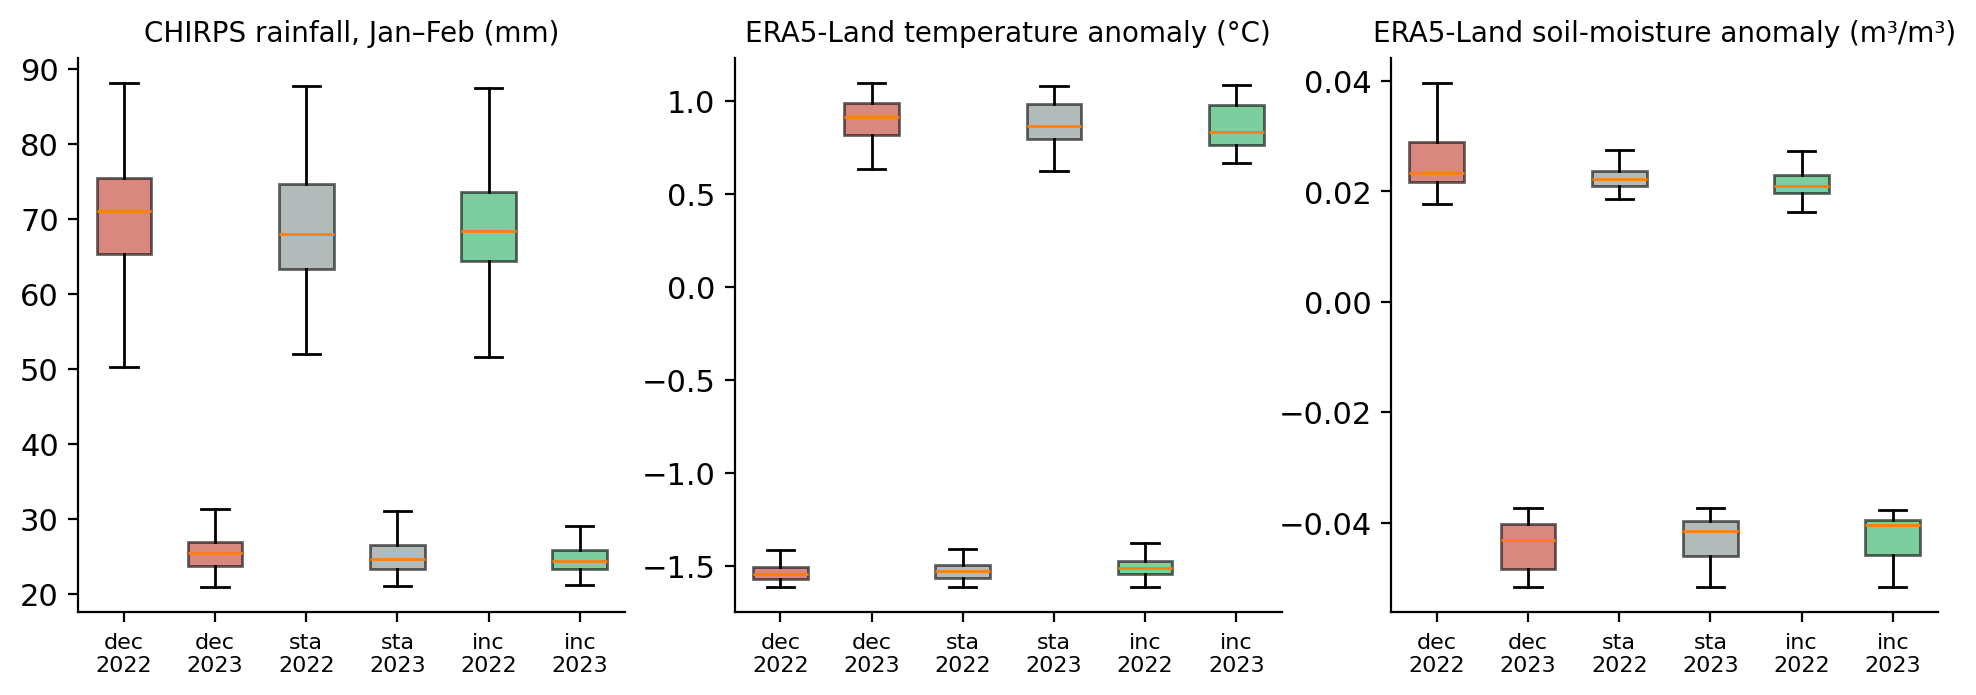
\includegraphics[width=\textwidth]{figures/fig_climate_by_class.png}
\caption{Rainfall, temperature anomaly and soil-moisture anomaly by class and year. The three classes are indistinguishable; only the year differs (\file{data/raw_metadata/selected_patches.csv}).}
\label{fig:climate}
\end{figure}

Climate values are attached to each patch by \texttt{reduce\_coarse}, which averages the coarse grid inside a square the size of one coarse pixel around the patch centre. The exported rainfall and ERA5 GeoTIFFs are therefore 1\,$\times$\,1 pixel.

\section{Source 5: terrain from NASADEM}

NASADEM is a reprocessed version of the elevation data from the Shuttle Radar Topography Mission (February 2000), at about 30\,m \citep{nasadem2020}. Earth Engine's \texttt{ee.Terrain.products} derives \textbf{slope} (steepness, degrees) and \textbf{aspect} (the direction a slope faces, degrees clockwise from north). Patch elevations range from 471 to 923\,m, mean slope is 6.4\dg, and only 19 patches have slopes of 12\dg{} or more.

\begin{whybox}
Terrain helps interpretation: steep slopes create shadows in optical images and distortions in radar images, and aspect affects moisture and therefore leaf fall. Terrain does not change within a year, so it is context, not evidence of change.
\end{whybox}

\section{The five sources at a glance}

\begin{table}[H]
\centering
\caption{The five data sources as used in the project. ``Export scale'' is the \texttt{scale} passed to Earth Engine (\file{src/gee_utils.py}).}
\label{tab:sources}
\small
\begin{tabularx}{\textwidth}{L{2.1cm}YYL{1.3cm}L{2.0cm}}
\toprule
Source & Earth Engine collection & Variables & Scale & Scenes / days \\
\midrule
Sentinel-2 L2A & \file{COPERNICUS/S2_SR_HARMONIZED} & 10 bands; NDVI, EVI, NDMI, NBR & 10\,m & 20 (T0), 23 (T1) \\
Sentinel-1 GRD & \file{COPERNICUS/S1_GRD} (IW, descending) & VV, VH (dB) & 10\,m & 15 (T0), 20 (T1) \\
CHIRPS & \file{UCSB-CHG/CHIRPS/DAILY} & rainfall total (mm) & 5,566\,m & 58 days each \\
ERA5-Land & \file{ECMWF/ERA5_LAND/MONTHLY_AGGR} & temperature and soil-moisture anomalies & 11,132\,m & Jan + Feb \\
NASADEM & \file{NASA/NASADEM_HGT/001} & elevation, slope, aspect & 30\,m & static \\
\bottomrule
\end{tabularx}
\end{table}

\begin{foryourreport}
\textbf{Study area} (about 400 words, with a map):
\begin{itemize}
  \item Location, districts, core/buffer/total area and forest types, citing \citet{kanha2026}.
  \item Why Kanha (handbook reasons) and why January--February.
  \item The rectangle's corners and area, and that it is larger than the reserve.
  \item A map: the whole of India (official boundary, not trimmed at the top), Madhya Pradesh, the reserve and the rectangle with patch points (your professor asks for this; see Chapter~\ref{ch:figures}).
\end{itemize}
\textbf{Data sources} (about 600 words):
\begin{itemize}
  \item Table~\ref{tab:sources} as a real table, with a citation for each source: \citet{drusch2012}, \citet{torres2012}, \citet{funk2015}, \citet{munozsabater2021}, \citet{nasadem2020}, and \citet{gorelick2017} for Earth Engine.
  \item Cloud masking, median composites, the harmonized collection, the descending orbit, only Sentinel-1A available.
  \item The four index equations (Equations~\ref{eq:ndvi}--\ref{eq:nbr}) with their citations, and the change definition (Equation~\ref{eq:delta}).
  \item The month-matched anomaly (Equation~\ref{eq:anomaly}).
\end{itemize}
\end{foryourreport}

\begin{selfcheck}
\begin{enumerate}
  \item Why does the project use the same two months in both years?
  \item Give the NDVI formula and say why a healthy canopy has a high NDVI.
  \item Why was the \emph{harmonized} Sentinel-2 collection needed for this project in particular?
  \item What is the difference between VV and VH, and which is more sensitive to vegetation?
  \item Radar backscatter fell by about 0.5\,dB everywhere. Why is this probably not forest loss?
  \item Why can rainfall not explain why one patch declined and its neighbour increased?
\end{enumerate}
\end{selfcheck}
